%!TEX root = ../thesis.tex
%*******************************************************************************
%****************************** Third Chapter **********************************
%*******************************************************************************
\chapter{ElecSim model}

% **************************** Define Graphics Path **************************
\ifpdf
    \graphicspath{{Chapter3/Figs/Raster/}{Chapter3/Figs/PDF/}{Chapter3/Figs/}}
\else
    \graphicspath{{Chapter3/Figs/Vector/}{Chapter3/Figs/}}
\fi

\section{Introduction}


The world faces significant challenges from climate change \cite{Masson-Delmotte2018}. A rise in carbon emissions increases the risk of severe impacts on the world such as rising sea levels, heat waves and tropical cyclones \cite{Masson-Delmotte2018}. A survey \cite{Cook2013} showed that 97\% of scientific literature concurs that the recent change in climate is anthropogenic.

High carbon emitting electricity generation sources such as coal and natural gas currently produce 65\% of global electricity, whereas low-carbon sources such as wind, solar, hydro and nuclear provide 35\% \cite{BP2018}. Hence, to bring about change and reach carbon-neutrality, a transition in the electricity mix is required.

% {\color{red}
% As shown by Figure \ref{fig:fuel_emissions_market_share}, the electricity mix is dominated by high carbon emitting fuels such as coal and natural gas. Low-carbon solutions, such as nuclear, renewables and hydro  produce less electricity put together than just coal.





% \begin{figure}
% 	\begin{center}

% 		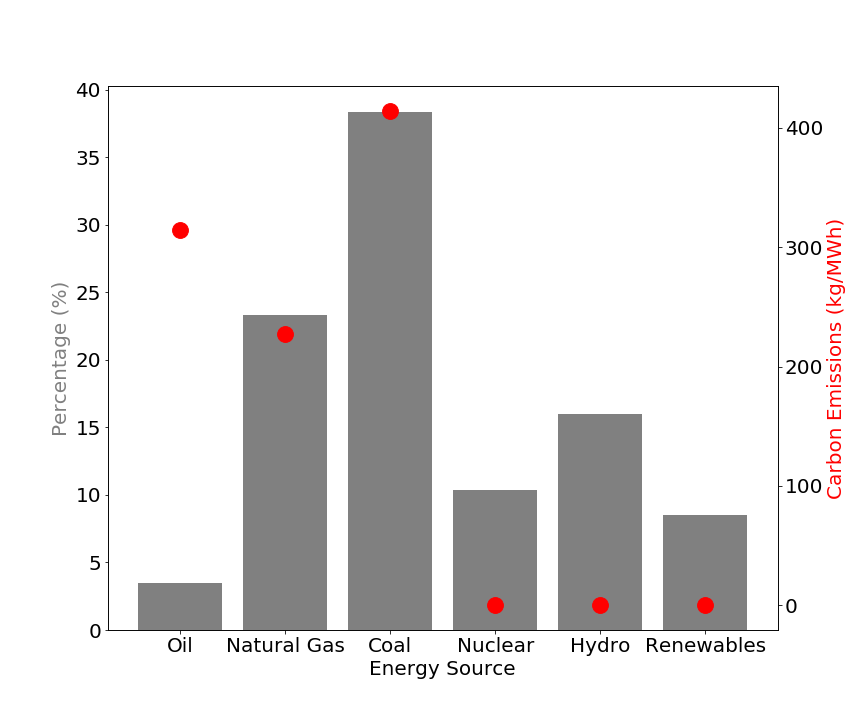
\includegraphics[width=0.45\textwidth]{figures/elec_gen_carbon.png}
% 		\caption{{\color{red}Global electricity generation sources and relative carbon emission intensity (2017). Bars refer to percentage of global electricity mix, and dots refer to carbon emission intensity}. ~\cite{BP2018,Hall1983}}
% 		\label{fig:fuel_emissions_market_share}
% 	\end{center}
% \end{figure}


% To achieve a low carbon energy infrastructure, and limit the effects of global warming, a transition in the electricity mix is required. Moving from a centralised and homogenous fossil fuel-based system to a distributed system based on renewable energy and batteries. Batteries are required due to the fact that most renewable sources are effected by conditions outside the control of the owners (e.g. time of day, wind speed and cloud cover). This leads to a need for electricity to be stored at times when renewable production exceeds renewable energy supply, and for the batteries to be discharged at times of high electrical demand and low renewable energy supply. 


% Such a transition needs to be performed in a safe and non-disruptive manner -- it may be possible to close down all fossil fuel plants in the next year, though if this leads to electricity shortages and power cuts then this is likely to cause significant problems both for companies and homes. Therefore a stepped approach which allows seamless transfer is desirable. This may seem a simple process to achieve -- slowly phase out existing fossil fuel generators and replace these by renewable sources -- however, there are many risks and uncertainties in this process. Existing power plants have an expected lifetime and their owners wish to maximise this and the profits which can be made from them, renewable sources are still developing -- meaning that their efficiency and reliability will change in years to come.
%  }

Due to the long construction times, operating periods and high costs of power plants, investment decisions can have long term impacts on future electricity supply \cite{Chappin2017}. Governments and society, therefore, have a role in ensuring that the negative externalities of emissions are priced into electricity generation. This is most likely to be achieved via carbon tax and regulation to influence electricity market players such as generation companies (GenCos).


Decisions made in an electricity markets may have unintended consequences due to their complexity. A method to test hypothesis before they are implemented would therefore be useful.

Simulation is often used to increase understanding as well as to reduce risk and reduce uncertainty. Simulation allows practitioners to realise a physical system in a virtual model. In this context, a model is defined as an approximation of a system through the use of mathematical formulas and algorithms. Through simulation, it is possible to test a system where real life experimentation would not be practical due to reasons such as prohibitively high costs, time constraints or risk of detrimental impacts. This has the dual benefit of minimising the risk of real decisions in the physical system, as well as allowing practitioners to test less risk-averse strategies.

Agent-based modelling (ABM) is a class of computational simulation models composed of autonomous, interacting agents and model the dynamics of a system. Due to the numerous and diverse actors involved in electricity markets, ABMs have been utilised in this field to address phenomena such as market power \cite{Ringler2016a}. 

This paper presents ElecSim, an open-source ABM that simulates GenCos in a wholesale electricity market. ElecSim models each GenCo as an independent agent and electricity demand. An electricity market facilitates trades between the two. 

GenCos make bids for each of their power plants. Their bids are based on the generator's short run marginal cost (SRMC) \cite{Perloff2012}, which excludes capital and fixed costs. The electricity market accepts bids in cost order, also known as merit-order dispatch. GenCos invest in power plants based on expected profitability.	

ElecSim is designed to provide quantitative advice to policy makers, allowing them to test policy outcomes under different scenarios. They are able to modify a script to realise a scenario of their choice. It can also be used by energy market developers who can test new electricity sources or policy types, enabling the modelling of changing market conditions.

% {\color{red}
% \begin{itemize}
% \item {\bf Policy experts} to test policy outcomes under different scenarios and provide quantitative advice to policy makers. They can provide a simple script defining the policies they wish to use along with the parameters for these polices.
% \item {\bf Energy market developers} who can use the extensible framework to add such things as new energy sources, policy types, consumer profiles and storage types. Thus allowing ElecSim to adapt to a changing ecosystem.
% \end{itemize}
% }



% \begin{figure}
% \centering
% 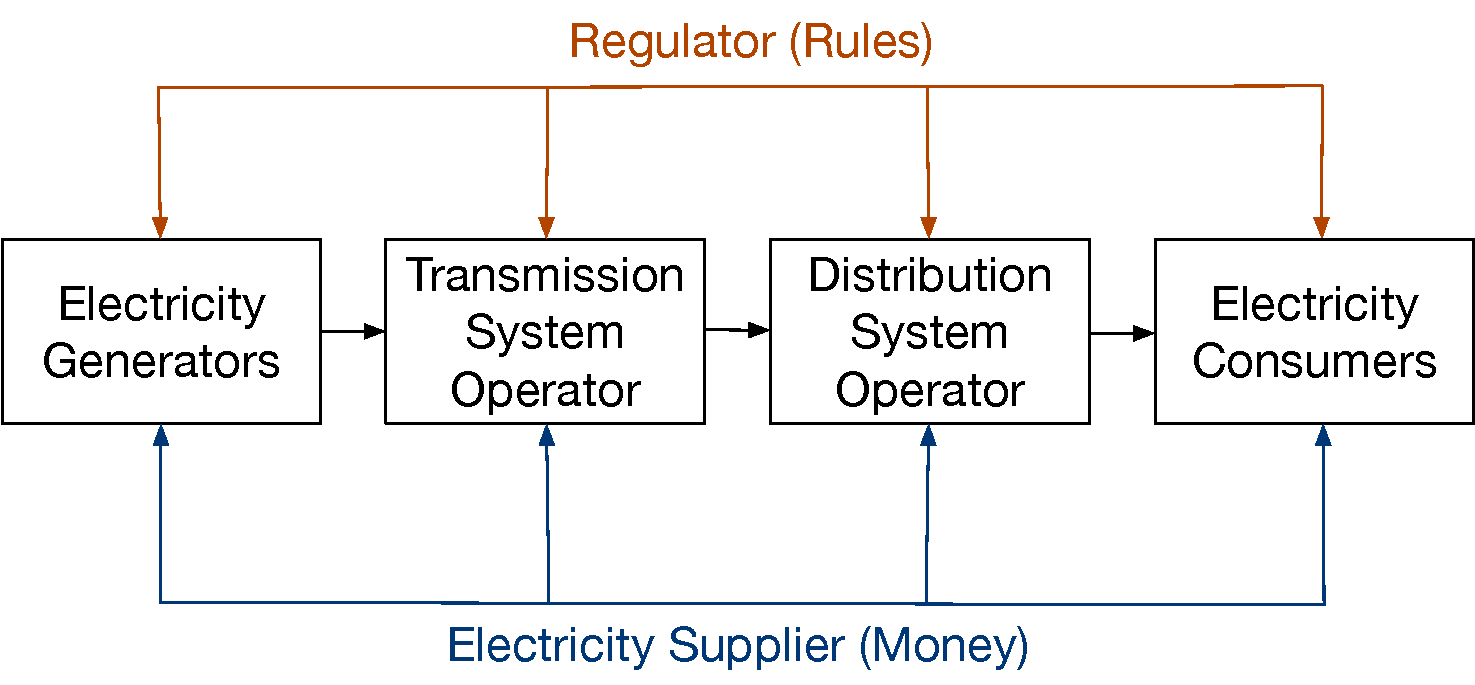
\includegraphics[width=0.9\linewidth]{figures/main_electricty_players}
% \caption{{\color{red}Schematic overview of the electricity system \cite{Erbach2016}.}}
% \label{fig:mainelectrictyplayers}
% \end{figure}



The contribution of this paper is a new open-source framework with example scenarios of varying carbon taxes. We provide curated data, and improve realism via Monte-Carlo sampling. Section \ref{Literature Review} is a literature review. Section \ref{Model} details the model and assumptions made, and Section \ref{Validation and Performance} provides performance metrics and validation. Section \ref{Scenario Testing} details our results. We conclude the work in Section \ref{Conclusion}.



\subsection{Literature Review}



Live experimentation of physical processes is often not practical. The costs of real life experimentation can be prohibitively high, and can require significant time in order to fully ascertain the long-term trends. There is also a risk that changes can have detrimental impacts and lead to risk-averse behaviour. These factors are true for electricity markets, where decisions can have long term impacts. Simulation, however, can be used for rapidly prototyping ideas. The simulation is parametrised by real world data and phenomena. Through simulation, the user is able to assess the likelihoods of outcomes under certain scenarios and parameters \cite{Law:603360}.



%\begin{table*}[]
%%	\begin{tabular}{|l|c|c|c|c|c|}
%	\begin{tabular}{lccccc} \toprule
%		\multicolumn{1}{c}{\textbf{Tool name}} & \textbf{Open Source} & \textbf{Long-Term Investment} & \textbf{Market} & \textbf{Stochastic Inputs} & \textbf{Country Generalisability} \\ \midrule
%		SEPIA \cite{Harp2000}  & \checkmark           & $\times$                             & \checkmark      & Demand                     & \checkmark                        \\ 
%		EMCAS ~\cite{Conzelmann}   & $\times$                    & \checkmark                    & \checkmark      & Outages                    & \checkmark                        \\ 
%		NEMSIM ~\cite{Batten2006}  & ?              & \checkmark                    & \checkmark      & $\times$                          & $\times$                                 \\ 
%		AMES  ~\cite{Sun2007} & \checkmark           & $\times$                             & Day-ahead       & $\times$                          & $\times$                                 \\ 
%		PowerACE ~\cite{Rothengatter2007} & $\times$                    & \checkmark                    & \checkmark      & Outages/Demand             & \checkmark                        \\ 
%		MACSEM  ~\cite{Praca2003}  & ?              & $\times$                             & \checkmark      & $\times$                          & \checkmark                        \\ 
%		GAPEX  ~\cite{Cincotti2013} & ?              & $\times$                             & Day-ahead       & $\times$                          & \checkmark                        \\ 
%		EMLab ~\cite{Chappin2017}  & \checkmark           & \checkmark                    & Futures         & $\times$                          & \checkmark                        \\ 
%		ElecSim                                  & \checkmark           & \checkmark                    & Futures         & \checkmark                 & \checkmark                        \\ \hline
%	\end{tabular}
%	\caption{Features of electricity market agent based model tools.}
%	\label{table:tool_comparison}
%\end{table*}


% {\color{red}Electricity energy policy modelling is an example where simulation can be used. Real-life experimentation of energy policy is not always feasible due to the long times required to observe results and high risks associated with setting a sub-optimal policy which could radically alter business models and lead to blackouts in electricity supply. Decisions can have long-term impacts, such as producing an electricity market with many expensive and highly polluting coal power plants, they may have ramp-up times, which is the time it takes for a generator to increase electricity production, that are not suitable to accommodate the intermittent electrical flow of renewables. Intermittent electrical flow is where sources of electricity exhibit uncontrolled increases or decreases in output, which is often the case for renewables such as wind, solar, wave and tidal \cite{Challenges2016}. A number of different simulations and computer models have been used to aid policy makers and energy market developers in coming to informed conclusions:}

Energy models can typically be classified as top-down macro-economic models or bottom-up techno-economic models~\cite{Bohringer1998}. Top-down models typically focus on behavioural realism with a focus on macro-economic metrics. They are useful for studying economy-wide responses to policies ~\cite{Hall2016}, for example MARKAL-MACRO \cite{Fishbone1981} and LEAP \cite{Heaps2016}. Bottom-up models represent the energy sector in detail, and are written as mathematical programming problems~\cite{Gargiulo2013}. %\vphantom{They detail technology explicitly, and can include cost and emissions implications~\cite{Hall2016}.}

It is possible to further categorise bottom-up models into optimisation and simulation models. Optimisation energy models minimise costs or maximise welfare, defined as the material and physical well-being of people ~\cite{Keles2017}. Examples of optimisation models are MARKAL/TIMES~\cite{Fishbone1981} and MESSAGE~\cite{Schrattenholzer1981}. % MARKAL is possibly the most widely used general purpose energy systems model~\cite{Pfenninger2014}.

However, electricity market liberalisation in many western democracies has changed the framework conditions. Centralised, monopolistic, decision making entities have given way to multiple heterogeneous agents acting for their own best interest~\cite{Most2010}. Policy options must therefore be used to encourage changes to attain a desired outcome. It is proposed that these complex agents are modelled using ABMs due to their non-deterministic nature. 


%Traditional centralised optimisation models are not designed to adequately describe a system which is out of equilibrium. They assume perfect foresight, and risk neutral investments, with no regulatory uncertainty, whilst, the core dynamics which emerge from equilibrium remain a black-box. A problem, for example, may be that the equilibrium model assumes a target will be reached, and will not provide the analyst with reasons for which this policy target will not be met. Reasons for this could be investment cycles, which are frequently observed in markets and would move the model away from the equilibrium \cite{Chappin2017}.

Traditional centralised optimisation models are not designed to  describe a system which is out of equilibrium. Optimisation models assume perfect foresight and risk neutral investments with no regulatory uncertainty. The core dynamics which emerge from equilibrium remain a black-box. For example, the model assumes a target will be reached, and does not provide information for which this is not the case. Reasons for this could be investment cycles which move the model away from equilibrium \cite{Chappin2017}.




% {\color{red}Agent-based simulation for electricity markets has received increasing attention in recent years. }

% {\color{red}There are numerous different mechanisms/markets for GenCos to sell electricity. These mechanisms can largely be split into pool markets and bilateral contracts. A pool market is a market in which bids and offers use supply and demand principles to set the price. Pool markets operators typically provide the function of matching buyers and sellers. Bilateral contracts are typically longer term markets where a GenCo will sell electricity to a demand company based on long-term contracts. }

% {\color{red} These mechanisms can be divided further into day-ahead markets and futures markets. Where day-ahead markets are markets where a buyer assesses how much energy it will need to meet demand the next day, and how much it is willing to pay for this volume, hour by hour \cite{nordpool_20192}. The seller (GenCo), will decide how much electricity it can deliver and at what price, hour by hour. Futures markets is where electricity is traded as a commodity, where electricity is bought at a certain price, at either high or low demand at a point in the future.}



%\begin{table}[]
%	%	\begin{tabular}{|l|c|c|c|c|c|}
%	\small	
%	\begin{tabular} 
%		
%		\multicolumn{1}{c}{\textbf{Tool name}} & \textbf{Open Source} & \textbf{Long-Term Investment} & \textbf{Market} & \textbf{Stochastic Inputs} & \textbf{Country Generalisability} \\ \midrule
%		SEPIA \cite{Harp2000}  & \checkmark           & $\times$                             & \checkmark      & Demand                     & \checkmark                        \\ 
%		EMCAS ~\cite{Conzelmann}   & $\times$                    & \checkmark                    & \checkmark      & Outages                    & \checkmark                        \\ 
%		NEMSIM ~\cite{Batten2006}  & ?              & \checkmark                    & \checkmark      & $\times$                          & $\times$                                 \\ 
%		AMES  ~\cite{Sun2007} & \checkmark           & $\times$                             & Day-ahead       & $\times$                          & $\times$                                 \\ 
%		GAPEX  ~\cite{Cincotti2013} & ?              & $\times$                             & Day-ahead       & $\times$                          & \checkmark                        \\ 
%		PowerACE \cite{Rothengatter2007} & $\times$                    & \checkmark                    & \checkmark      & Outages Demand             & \checkmark                        \\ 
%		
%		EMLab ~\cite{Chappin2017}  & \checkmark           & \checkmark                    & Futures         & $\times$                          & \checkmark                        \\ 
%		MACSEM  ~\cite{Praca2003}  & ?              & $\times$                             & \checkmark      & $\times$                          & \checkmark                        \\ 
%		ElecSim                                  & \checkmark           & \checkmark                    & Futures         & \checkmark                 & \checkmark                        \\ \hline
%	\end{tabular}
%	\caption{Features of electricity market ABM tools.}
%	\label{table:tool_comparison}
%	\vskip -1cm
%\end{table}


A number of ABM tools have emerged over the years to model electricity markets: SEPIA~\cite{Harp2000}, EMCAS~\cite{Conzelmann}, NEMSIM~\cite{Batten2006}, AMES~\cite{Sun2007}, GAPEX~\cite{Cincotti2013}, PowerACE~\cite{Rothengatter2007}, EMLab~\cite{Chappin2017} and MACSEM ~\cite{Praca2003}. Table \ref{table:tool_comparison} shows that these do not suit the needs of an open source, long-term market model. We will demonstrate that Monte-Carlo sampling of parameters is also required to increase realism.

There have been a number of recent studies using ABMs which focus on electricity markets, however they often utilize ad-hoc tools which are designed for a particular application \cite{Saxena2019, hadar2019, Kunzel2018}. ElecSim, however, has been built for re-use and reproducibility. The survey \cite{Weidlich2008} cites that many of these tools do not release source code or parameters, which is a problem that ElecSim seeks to address.

Table \ref{table:tool_comparison} contains six columns: tool name, whether the tool is open source or not, whether they model long-term investment in electricity infrastructure, and the markets they model. We determine how the stochasticity of real life is modelled, and determine whether the model is generalisable to different countries. 


An open source toolkit is important for reproducibility, transparency and lowering barriers to entry. It enables users to expand the model to their requirements and respective country. The modelling of long-term investment enables scenarios to emerge, and enable users to model investment behaviour. We demonstrate that the use of a Monte-Carlo method improves results.

SEPIA \cite{Harp2000} is a discrete event ABM which utilises Q-learning to model the bids made by GenCos. SEPIA models plants as being always on, and does not have an independent system operator (ISO), which in an electricity market, is an independent non-profit organization for coordinating and controlling of regular operations of the electric power system and market \cite{Zhou2007}. SEPIA does not model a spot market, instead focusing on bilateral contracts. As opposed to this, ElecSim has been designed with a merit-order, spot market in mind. As shown in Table \ref{table:tool_comparison}, SEPIA does not include a long-term investment mechanism. 

EMCAS ~\cite{Conzelmann} is a closed source ABM. EMCAS investigates the interactions between physical infrastructures and economic behaviour of agents. However, ElecSim focuses on the dynamics of the market, and provides a simplified, transparent model of market operation, whilst maintaining robustness of results.

NEMSIM \cite{Grozev2005} is an ABM that represents Australia's National Electricity Market (NEM). Participants are able to grow and change over time using learning algorithms. NEMSIM is non-generalisable to other electricity markets, unlike ElecSim.

AMES ~\cite{Sun2007} is an ABM specific to the US Wholesale Power Market Platform and therefore not generalizable for other countries. GAPEX \cite{Cincotti2013} is an ABM framework for modelling and simulating power exchanges . GAPEX utilises an enhanced version of the reinforcement technique Roth-Erev \cite{RothAE1995} to consider the presence of affine total cost functions. However, neither of these model the long-term dynamics for which ElecSim is designed.



PowerACE ~\cite{Rothengatter2007} is a closed source ABM of electricity markets that integrates short-term daily electricity trading and long-term investment decisions. PowerACE models the spot market, forward market and a carbon market. Similarly to ElecSim, PowerACE initialises GenCos with each of their power plants. However, as can be seen in Table \ref{table:tool_comparison}, unlike ElecSim, PowerACE does not take into account stochasticity of price risks in electricity markets ~\cite{Most2010}.

EMLab ~\cite{Chappin2017} is an open-source ABM toolkit for the electricity market. Like PowerACE, EMLab models an endogenous carbon market, however, they both differ from ElecSim by not taking into account stochasticity in the electricity markets, such as in outages, fuel prices and operating costs. After correspondence with the authors, however, we were unable to run the current version.

MACSEM \cite{Praca2003} has been used to probe the effects of market rules and conditions by testing different bidding strategies. MACSEM does not model long term investments or stochastic inputs.


As can be seen from Table \ref{table:tool_comparison}, none of the tools fill each of the characteristics we have defined. We therefore propose ElecSim to contribute an open source, long-term, stochastic investment model. 






\subsection{Second subsection in the first section}
\dots and some more \dots

\subsubsection{First subsub section in the second subsection}
\dots and some more in the first subsub section otherwise it all looks the same
doesn't it? well we can add some text to it \dots

\subsection{Third subsection in the first section}
\dots and some more \dots

\subsubsection{First subsub section in the third subsection}
\dots and some more in the first subsub section otherwise it all looks the same
doesn't it? well we can add some text to it and some more and some more and
some more and some more and some more and some more and some more \dots

\subsubsection{Second subsub section in the third subsection}
\dots and some more in the first subsub section otherwise it all looks the same
doesn't it? well we can add some text to it \dots

\section{Second section of the third chapter}
and here I write more \dots

\section{The layout of formal tables}
This section has been modified from ``Publication quality tables in \LaTeX*''
 by Simon Fear.

The layout of a table has been established over centuries of experience and 
should only be altered in extraordinary circumstances. 

When formatting a table, remember two simple guidelines at all times:

\begin{enumerate}
  \item Never, ever use vertical rules (lines).
  \item Never use double rules.
\end{enumerate}

These guidelines may seem extreme but I have
never found a good argument in favour of breaking them. For
example, if you feel that the information in the left half of
a table is so different from that on the right that it needs
to be separated by a vertical line, then you should use two
tables instead. Not everyone follows the second guideline:

There are three further guidelines worth mentioning here as they
are generally not known outside the circle of professional
typesetters and subeditors:

\begin{enumerate}\setcounter{enumi}{2}
  \item Put the units in the column heading (not in the body of
          the table).
  \item Always precede a decimal point by a digit; thus 0.1
      {\em not} just .1.
  \item Do not use `ditto' signs or any other such convention to
      repeat a previous value. In many circumstances a blank
      will serve just as well. If it won't, then repeat the value.
\end{enumerate}

A frequently seen mistake is to use `\textbackslash begin\{center\}' \dots `\textbackslash end\{center\}' inside a figure or table environment. This center environment can cause additional vertical space. If you want to avoid that just use `\textbackslash centering'


\begin{table}
\caption{A badly formatted table}
\centering
\label{table:bad_table}
\begin{tabular}{|l|c|c|c|c|}
\hline 
& \multicolumn{2}{c}{Species I} & \multicolumn{2}{c|}{Species II} \\ 
\hline
Dental measurement  & mean & SD  & mean & SD  \\ \hline 
\hline
I1MD & 6.23 & 0.91 & 5.2  & 0.7  \\
\hline 
I1LL & 7.48 & 0.56 & 8.7  & 0.71 \\
\hline 
I2MD & 3.99 & 0.63 & 4.22 & 0.54 \\
\hline 
I2LL & 6.81 & 0.02 & 6.66 & 0.01 \\
\hline 
CMD & 13.47 & 0.09 & 10.55 & 0.05 \\
\hline 
CBL & 11.88 & 0.05 & 13.11 & 0.04\\ 
\hline 
\end{tabular}
\end{table}

\begin{table}
\caption{A nice looking table}
\centering
\label{table:nice_table}
\begin{tabular}{l c c c c}
\hline 
\multirow{2}{*}{Dental measurement} & \multicolumn{2}{c}{Species I} & \multicolumn{2}{c}{Species II} \\ 
\cline{2-5}
  & mean & SD  & mean & SD  \\ 
\hline
I1MD & 6.23 & 0.91 & 5.2  & 0.7  \\

I1LL & 7.48 & 0.56 & 8.7  & 0.71 \\

I2MD & 3.99 & 0.63 & 4.22 & 0.54 \\

I2LL & 6.81 & 0.02 & 6.66 & 0.01 \\

CMD & 13.47 & 0.09 & 10.55 & 0.05 \\

CBL & 11.88 & 0.05 & 13.11 & 0.04\\ 
\hline 
\end{tabular}
\end{table}


\begin{table}
\caption{Even better looking table using booktabs}
\centering
\label{table:good_table}
\begin{tabular}{l c c c c}
\toprule
\multirow{2}{*}{Dental measurement} & \multicolumn{2}{c}{Species I} & \multicolumn{2}{c}{Species II} \\ 
\cmidrule{2-5}
  & mean & SD  & mean & SD  \\ 
\midrule
I1MD & 6.23 & 0.91 & 5.2  & 0.7  \\

I1LL & 7.48 & 0.56 & 8.7  & 0.71 \\

I2MD & 3.99 & 0.63 & 4.22 & 0.54 \\

I2LL & 6.81 & 0.02 & 6.66 & 0.01 \\

CMD & 13.47 & 0.09 & 10.55 & 0.05 \\

CBL & 11.88 & 0.05 & 13.11 & 0.04\\ 
\bottomrule
\end{tabular}
\end{table}
